\documentclass[10pt,twocolumn,twoside]{gsajnl}
\articletype{inv} % article type: {inv} Investigation

\usepackage{breqn}

\usepackage{subcaption}

\newcommand{\EQ}[1]{Eq.~\eqref{eq:#1}}
\newcommand{\EQS}[2]{Eqs.~\eqref{eq:#1} and \eqref{eq:#2}}
\newcommand{\FIG}[1]{Fig.~\ref{fig:#1}}
\newcommand{\TAB}[1]{Tab.~\ref{tab:#1}}
\newcommand{\REF}[1]{ref.~\citep{#1}}

\newcommand{\jcomment}[2][noinline]{\todo[size=\tiny,author=JVC,color=red,#1,caption={},fancyline]{#2}}

%%% math macros
\DeclareMathOperator*{\argmin}{arg\,min}
\newcommand{\pfix}{p_{\mathrm{fix}}}

\usepackage{setspace}

%%%%%%%%%%%%%%%%%%%%%%%%%%%%%%%%%%%%%%%%%%%%%%%%%%%%%%%%%%%%%%%%%%%%%%%%%%%%%%
\title{Genetic draft and valley crossing}
\author[$\ast$]{Taylor Kessinger}
\author[$\ast$,1]{Jeremy Van Cleve}
\affil[$\ast$]{Department of Biology, University of Kentucky}

\keywords{genetic drift; rapid adaptation; epistasis; fitness landscape}
\runningtitle{Genetic draft and valley crossing}
\runningauthor{Kessinger and Van Cleve}

\begin{abstract}
Living systems are characterized by complex adaptations which require multiple coordinated mutations in order to function. Empirical studies of fitness landscapes that result from the many possible mutations in a gene region reveal many fitness peaks and valleys that connect them. Thus, it is possible that some complex adaptations have arisen by evolutionary paths whose intermediate states are neutral or even deleterious.
When intermediates are deleterious, traversing such an evolutionary path is known as ``crossing a fitness valley".
Previous efforts at studying this problem have rigorously characterized the rate at which such complex adaptations evolve in populations of roughly equally fit individuals.
However, populations that are very large or have broad fitness distributions, such as many microbial populations, adapt quickly, which substantially alters the fate and dynamics of individual mutations due to the action of genetic draft.
We investigate the rate at which complex adaptations evolve in these rapidly adapting populations in regions without recombination.
We confirm that rapid adaptation overall increases the time required to cross a valley; however, rapid adaptation can make it easier for deeper valleys to be crossed relative to the time required for single beneficial mutations to sweep to fixation.
\end{abstract}

%%%%%%%%%%%%%%%%%%%%%%%%%%%%%%%%%%%%%%%%%%%%%%%%%%%%%%%%%%%%%%%%%%%%%%%%%%%%%%

\begin{document}

\maketitle
\thispagestyle{firststyle}
\marginmark
\firstpagefootnote

\correspondingauthoraffiliation{1}{Corresponding author: Department of Biology, University of Kentucky. E-mail: \href{emailto:jvancleve@uky.edu}{jvancleve@uky.edu}}

%%%%%%%%%%%%%%%%%%%%%%%%%%%%%%%%%%%%%%%%%%%%%%%%%%%%%%%%%%%%%%%%%%%%%%%%%%%%%% 

\begin{spacing}{1.5}

\section{Introduction}

The simplest adaptive scenarios in evolution involve the arisal and fixation of successive beneficial mutations.
This appears to be how Darwin thought even complex systems, such as the vertebrate eye, evolved \citep{darwin_1859}, and this assumption underlies many models in evolutionary theory including those from adaptive dynamics \citep{Geritz:Kisdi:1998,Dercole:Rinaldi:2008} and theories of adaptation \citep{Gillespie:1983,Orr:1998,Gillespie:1991}.
Evolution will proceed in this fashion if there always exists a sequence of mutations from an initial genotype to the high fitness genotype in which each mutant genotype in the sequence has a higher fitness than the previous one.
If the individual fitness of each genotype is visualized as a surface or landscape wherein the axes represent alternative alleles at each locus, then smooth landscapes with a single peak ensure that uphill paths exist no matter where a population starts.
However, many empirical fitness landscapes are not completely smooth and have multiple peaks \citep[reviewed in][]{Szendro:Schenk:2013,Visser:Krug:2014,Obolski:Ram:2018}.
In such landscapes, wild type individuals may have to traverse a mutational valley--a region of lower fitness--in order to reach a higher fitness peak.
This is a special case of ``sign epistasis".
We seek to characterize this ``valley crossing" process in order to better understand the routes adaptation is likely to take on these rugged empirical landscapes \citep[e.g.,][]{Aguilar-Rodriguez:Payne:2017} and to assess the likelihood of valley crossing under more complex scenarios in which it may in fact be common \citep[e.g.][]{trotter_2014}.

Valley crossing in asexual populations is increasingly well understood \citep{weissman_2009}.
If the number of mutants produced every generation is high, as is the case in large populations with high mutation rates, a complex adaptation requiring multiple mutations that is destined to fix will eventually be generated \emph{de novo}.
This is sometimes called deterministic fixation of the multiple mutant \citep{weissman_2009}.
In small populations, neutral or deleterious intermediate mutants generated by wild type individuals can drift to fixation. Further mutations necessary for the adaptation can then arise on intermediate mutant backgrounds and fix due to positive selection.
This is the sequential fixation regime \citep{weissman_2009}.
A third possibility occurs for intermediate population sizes wherein wild type individuals generate transient mutant subpopulations or ``bubbles".
These bubbles are ordinarily doomed to extinction due to drift, but additional mutations in a lucky bubble may generate a complex adaptation that sweeps to fixation; this process has been referred to as ``tunneling" \citep{iwasa_2004, weissman_2009}.
On its own, valley crossing becomes more likely as the population size increases \citep{weissman_2009}.
However, recent work suggests that valley crossing relative to the fixation of a simple beneficial mutation is least likely at intermediate population sizes in which tunneling occurs \citet{ochs_2015}.
This suggests that tunneling may be the most difficult mode of valley crossing. 
Recombination also affects the rate of valley crossing.
Infrequent recombination decreases valley crossing times \citep{weissman_2010}.
At high values of the recombination rate, however, individuals carrying the full complex adaptation outcross with the wild type and produce deleterious intermediates that retard the growth of the multiple mutant.
An additional effect that can heighten the rate at which valley crossing occurs is population subdivision \citep{Bitbol:Schwab:2014}: the population size within a subdivision is smaller, meaning that selection against potentially harmful intermediates is relaxed.
Intermediates can then drift to high frequency or even fixation, increasing the rate at which complex adaptations arise.

Previous studies of valley crossing focus primarily on populations where all individuals are equal in fitness except for the focal loci, i.e., the loci at which the individual mutations comprising the complex adaptation segregate.
This is tantamount to assuming that variation in the background fitness of the population is negligible.
In such populations, genetic drift governs the fate of neutral alleles, as well as the behavior of deleterious or beneficial alleles where they are rare (close to frequency zero) or common (close to frequency one).
Alleles whose dynamics are primarily determined by genetic drift can be effectively modeled by a diffusion approximation \citep{Wright:1945,Kimura:1955,Kimura:1957}, and the ancestry of a population in the absence of selection is described well by the classic Kingman coalescent \citep{Kingman:1982}, where pairs of branches in the genealogy merge back in time until the most recent common ancestor.
When population sizes are very large or the fitness variation in the population is substantial, however, the behavior of genetic variation is governed more by genetic \emph{draft} than by genetic drift \citep{gillespie_2000, gillespie_2001, masel_2011, neher_shraiman_2011}.
Broadly speaking, drift results from the fact that each generation is imperfectly sampled from the previous generation.
Draft, on the other hand, is the sum of hitchhiking effects due to selection on sites linked to the focal loci.
The standard technique of defining a reduced ``effective population size" fails to capture several fundamental qualitative differences between drift and draft.
For example, new mutations in a drafting population can rapidly be brought to high frequency, and the variance in offspring number almost diverges \citep{neher_shraiman_2011}.
Drafting populations commonly have genealogies in which more than two branches merge at once (or almost at once) and that are better described by alternative coalescent processes such as the Bolthausen-Sznitman coalescent \citep{neher_hallatschek_2013, brunet_2007, schweinsberg_2017}.
Additionally under genetic draft, the frequency spectrum of neutral alleles is non-monotonic, with a marked uptick near frequency one--or, equivalently, a depression in intermediate frequency alleles, which are quickly swept out of the population \citep{neher_shraiman_2011,kosheleva_2013,neher_hallatschek_2013}.
Only a handful of individuals near the ``nose" of the fitness distribution are likely to persist, and they give rise to the bulk of the future population and carry linked alleles with them.
The parameter that determines whether drift or draft is more important is the product of the population size $N$ and the standard deviation in fitness $\sigma$ \citep{neher_hallatschek_2013}.

It is increasingly realized that draft may play a critical role in shaping genetic diversity, especially in many microbial species, where population sizes can be large but ``effective population sizes" are many orders of magnitude smaller \citep{masel_2011}.
The possibility that neutral variants are affected more strongly by selection at linked sites than by genetic drift, even in organisms like \emph{Drosophila}, is one possible explanation for the ``paradox of variation", the fact that genetic diversity and population size often do not scale linearly \citep{gillespie_2000, gillespie_2001, neher_kessinger_2013, corbett-detig_2015}.
Draft likewise may have profound effects on the evolution of complex adaptations.
Preliminary evidence for this comes from \citet{neher_shraiman_2011}, who explored how draft affects valley crossing via stochastic tunneling by calculating the mutant bubble size distribution in a rapidly adapting facultatively sexual population.
They found that, compared to drift, draft generally causes the distribution of bubble sizes to drop off more quickly, meaning that bubbles tend to be smaller overall: however, as the mutant lineage's fitness is determined not only by a mutation's intrinsic fitness effect but also the genetic background on which it appears, the fitness effect of a focal mutation plays less of a role in capping the size of the lineage.
Thus, while draft may make valley crossing via tunneling more difficult, the total effect is not immediately obvious.
Here, we extend these results by studying how genetic draft in asexual populations affects the rate of crossing fitness valleys across a range of population sizes, including ones in which tunneling is not the dominant mode of valley crossing.

The complicating factor is that, in an asexual population, the dynamics are governed almost entirely by what happens in the nose of the fitness distribution, and these dynamics can be highly stochastic.
In previous approaches, these stochastic effects were smoothed due to the presence of recombination \citep{neher_shraiman_2011, neher_shraiman_2009}: the critical nose dynamics are still important in a sexual population, but the fitness distribution is more Gaussian overall.
Moreover, a full understanding of the behavior of complex adaptations requires that one consider the dynamics of individual lineages.
The equations that describe said dynamics, however, are very difficult to solve; \citet{neher_shraiman_2011} were able to circumvent this issue by carefully choosing a recombination model that allowed them to avoid the need to directly solve these equations.
We therefore must focus primarily on simulation approaches, as analytical solutions for the behavior of a mutation in the nose of an asexual population are very difficult to obtain.
We expand on the work of \citet{neher_shraiman_2011} by considering not only stochastic tunneling but also sequential fixation; in fact, we find that, over a significant chunk of parameter space, stochastic tunneling effectively \emph{does not happen} in drafting populations, and sequential fixation appears to be the dominant mode of valley crossing.
We also show that fitness valley crossing occurs at an overall lower rate in rapidly adapting populations.
This is consistent with the fact that clonal interference and genetic background effects retard the growth of fit mutant lineages, slowing the expansion of a beneficial mutation.
In addition, we confirm that in rapidly adapting populations, adaptive fixations of alleles are more likely to be complex adaptations involving a fitness valley than they are in populations where genetic drift is the primary force shaping genetic variation at linked sites; essentially, genetic draft maintains the linkage that makes it possible to leap across fitness landscapes rather than adapt primarily by climbing to local peaks.
These observations add to the growing intuition that complex adaptations that involve evolution across fitness valleys may not be a surprising result of the evolutionary process but rather an expected one.

\section{Mathematical background}

\begin{figure}[t]
\begin{center}
  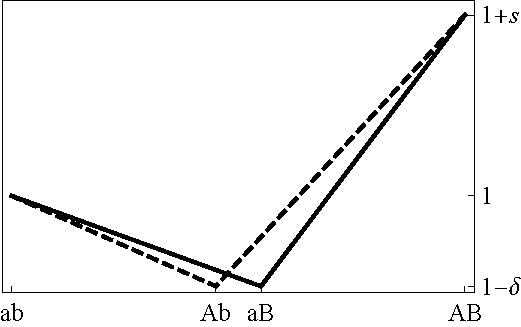
\includegraphics[scale=0.75]{Figures/valley.pdf}
  \caption{Fitness landscape.}
  \label{fig:landscape}
\end{center}
\end{figure}

Our model features a population of $N$ haploid individuals in which an effectively infinite number of ``background" loci, with weak fitness effects, are currently segregating.
A complex adaptation can occur in the population via mutations at two ``focal" loci (which are treated separately from the background loci).
The mutation rate is $\mu_1$ at the first focal locus and $\mu_2$ at the second locus.
Individuals who are mutant at one locus and wild-type at the other have reduced fitness relative to the wild type, but the double mutant state corresponds to a ``complex" adaptation that increases fitness.
For simplicity, we assume that individuals must mutate at the first locus \emph{before} they can mutate at the second locus, so that $\mu_1$ is the mutation rate into the deleterious intermediate state and $\mu_2$ is the mutation rate toward the full complex adaptation.
The fitnesses of these states are $1-\delta$ and $1+s$, respectively, with $\delta \leq 0$ and $1/N < s \ll 1$ (so-called ``strong selection").
This setup closely mirrors that of \citep{weissman_2009}.

We further assume that the large number of background loci of weak effect contribute to a constant background fitness variance $\sigma^2$.
Let $x$ be the background fitness of a lineage.
If the number of background loci is large, the distribution of background fitnesses $f(x)$ will generally be a series of (Dirac) $\delta$ functions, but its ensemble average will be roughly Gaussian \citep{good_2014}: $f(x) \approx \frac{1}{\sqrt{2\pi}\sigma} \exp (\frac{(x-\bar{x})^2}{2\sigma^2})$.
By Fisher's ``fundamental theorem", the mean fitness $\bar{x}$ will advance due to selection at a rate equal to $\sigma^2$: the total rate of advance will depend also on contributions from drift and the average effect of mutations.

Given this background fitness distribution, we are interested in the expected time $\mathbb{E}\left[ T\right]$ for a beneficial double mutant at the focal loci (a ``complex adaptation'') to arise and fix in the population.
We emphasize that $\sigma^2$ is only a \emph{background} fitness variance and does not include the effects of the focal loci.
For the most part, we assume that mutations at the focal loci are either at low enough frequency, so that they do not substantially affect the total fitness variance, or that they are on the way to fixation, and hence the population is destined to become fixed at those loci.

\citet{weissman_2009} divided the possible modes of asexual valley crossing into several distinct regimes.
We classify them, broadly, as \emph{sequential fixation}, \emph{deterministic fixation}, and \emph{stochastic tunneling}.
What follows is a brief outline of the process of valley crossing in each of these regimes, as well as how these are likely to differ in our model.
We then present results for valley crossing times using forward-time simulations across a range of parameter values that includes each of these major regimes.

The \emph{sequential fixation} regime arises at small population sizes.
The wait time $\mathbb{E}\left[ T\right]$ can be partitioned into two components: the time $\tau_1$ until an intermediate mutation arises \emph{that is destined to fix} and the time $\tau_2$ until the complex adaptation arises and is likewise destined to fix.
$\tau_1$ is one divided by the rate $N\mu_1 p$ at which intermediate mutants arise that are destined to fix: on average, $N\mu_1$ mutants appear every generation, and the diffusion approximation yields $p = (e^\delta - 1)/(e^{N\delta} - 1)$.
$\tau_2$, similarly, is approximately one divided by $N\mu_2 s$ and in general will be dwarfed by $\tau_1$.
When genetic draft is more important than genetic drift, $p$ in $\tau_1$ takes on a much more complicated form similar to that in \citet{good_2014}: in general, the dependence on $\delta$ is lessened provided that $\sigma \gtrsim \delta$, as deleterious mutations that arise on significantly fitter than average backgrounds can be destined to fix.
$\tau_2$ likewise has lessened dependence on $s$, as a complex adaptation that does \emph{not} arise on a fitter-than-average background lineage may be doomed to extinction.

The process of \emph{deterministic fixation} occurs when the number of single mutants introduced every generation is sufficiently large: $N\mu_1 \gg 1$.
One possibility is that the intermediate exists in what is roughly mutation-selection balance, so that it persists at a low frequency.
Lucky complex adaptations can then arise on this background of roughly constant intermediate influx, then sweep to fixation.
This is known as \emph{semi-deterministic tunneling}; we class it under the ``deterministic" umbrella because it is not necessary to consider the stochastic dynamics of individual deleterious mutant lineages.
Switching from drift to draft will affect the likelihood that a particular complex adaptation will sweep to fixation, but it seems unlikely to affect the mutation-selection balance dynamics for intermediates.
The strictest ``deterministic fixation" case occurs when $N \gg 2s/\pi \mu_1 \mu_2$.
In this case, multiple complex adaptations are likely to arise on independent backgrounds, and there is no guarantee that the first one to reach significant frequency will sweep through the population on its own.
In the draft case, we expect the fixation time to be increased due to the blunting effect of the genetic background.
However, note that the $N \gg 2s/\pi \mu_1 \mu_2$ cutoff is generally very large: for $\mu_1 = \mu_2 = 10^{-4}$ and $s = 0.1$, we have $N \approx 10^7$, a size that will prove difficult to probe with our simulation model.

Finally, we consider the intermediate case: \emph{stochastic tunneling}.
This process has three major components.
First, a single mutant lineage must appear, which occurs with rate $N\mu$.
If this lineage arises at time $t_0$ and persists until time $T$, then it gives rise to $W = \int_{t_0}^T n(t) dt$ total individuals before going extinct, where $n(t)$ is the number of mutant individuals extant at time $t$.
As in the introduction, we refer to such a short-lived mutant lineage, and all the individuals generated within that lineage, as a mutant ``bubble": the time integrated number of individuals $W$ is the ``weight" of the bubble.
If it establishes, the complex adaptation will quickly sweep to fixation.
The first two steps can be folded in together and considered as one process, so that what is relevant is the expected time until a single mutant lineage arises that is destined to produce a successful double mutant.
In this way, $\mathbb{E}\left[ T \right] = \mathbb{E} \left[ T_0 + T_1 \right]$, where $T_0$ is the time to the first successful bubble--the first that produces a double mutant that is destined for fixation--and $T_1$ is the time required for the double mutant to sweep.
We assume that $T_0 \gg T_1$, so that the wait time is dominated by the first term: in the drift case, the time required for $T_1$ to establish will be of order $1/s$ \citep{desai_fisher_2007}, and the sweep time will be of order $1/s \log (Ns)$, but $T_0$ can be many orders of magnitude greater.

This process is well understood in the drift case, and at first brush it seems possible to extend this understanding to the draft case.
Most of the time, a bubble will simply arise and go extinct.
If mutation and fixation are sufficiently rare events, then fixation of the double mutant can be modeled as a Poisson process: with probability $1-e^{-\mu \pfix W}$, the bubble with total size $W$ will give rise to a successful double mutant.
Computing the expected value of this quantity over all bubble sizes, $\phi = \left< 1-e^{\mu \pfix W} \right>$, gives the probability that some bubble will lead to a successful valley crossing.
In the draft case, the expected bubble size and fixation probability will both turn out to depend on the background fitness of an individual.
That is to say, it is not possible to simply compute $\pfix$ and the weight distribution by themselves, but rather one must convolute both of them over the background fitness.
Individuals whose background fitness is near the nose of the fitness distribution will tend to give rise to longer-lived lineages, and if those individuals give rise to the complex adaptation, it will therefore likewise be more likely to fix.
Thus, the distribution of $W$ will depend on the background fitness $x$ and the valley depth $\delta$, and $\pfix$ will depend on $x$ and the peak height $s$.
Once $\phi$ is obtained, it will have to be integrated over the fitness distribution $f(x)$ in order to obtain the total crossing probability $\upPhi(s,\delta) = \int_{-\infty}^\infty \phi(x,s,\delta) f(x) dx$.
The expected valley crossing time would then be $1/N\mu\upPhi$.

Unfortunately, a number of complicating factors prevent a full analytical description of this process.
First, $\pfix$ will not depend solely on the background fitness $x$ of a lineage.
Individuals in each lineage will accumulate mutations, broadening the fitness distribution \emph{of that lineage}, so $\pfix$ will depend specifically on the background fitness of the precise individual within said lineage that gives rise to the complex adaptation.
This issue can be swept aside by assuming that bubbles do not last long enough for their own distribution of fitnesses to become very broad.
The second issue is somewhat more severe: there is no principled way to compute the Laplace transform of the bubble size distribution.
Previous approaches such as \citet{weissman_2009} and \citet{neher_shraiman_2011} have relied on branching process approximations.
The latter in particular were able to derive the asymptotics of the bubble size distribution in a facultatively sexual population: they began by deriving a master equation for the distribution of bubble sizes with a birth rate that decreases in time as the mean fitness advances.
However, they relied on a recombination model that allowed them to directly obtain the integrated Laplace transform $\int_{-\infty}^\infty p(x) \phi(x) dx$ without the need to explicitly solve the branching process model; our model being an asexual one, this option is not available to us.
\iffalse
In addition, they evaded the need to send time to infinity in the model.
In principle this is necessary to integrate over all possible bubble sizes: but in practice, because the birth rate of a lineage decreases with time, this would yield the absurd result that $\phi$ itself decreases with time.
\fi
Since it seems unlikely that analytical approaches will yield a principled way of approximating the valley crossing time in the drift case, we focus on simulation methods to estimate the valley crossing time.


\iffalse
We begin by considering the dynamics of $\pfix(x,s)$ before moving on to consider the distribution of bubble sizes.
We focus on the case where background mutations are frequent but of weak effect--that is, the mean effect of background mutations $\bar{\epsilon}$ is small compared to $\sigma$, but background mutations occur at a high rate $U_b$.
\citet{hallatschek_2011} and \citet{good_2014} showed that the fixation probability in this regime obeys the differential equation 
\begin{equation}
v\partial_x \pfix(x,s) = x \pfix(x,s) + \frac{U_b\bar{\epsilon}^2}{2}\partial_x^2 \pfix(x,s) - \frac{\pfix(x,s)^2}{2},
\end{equation}
in which we have further assumed that $v \approx \sigma^2$, which is tantamount to claiming that mutational effects are less important than selection in determining the advance of the mean fitness.
For a neutral mutation ($s = 0$), the fixation probability is effectively zero at low $x$ but increases exponentially up until $x_c$, at which it becomes roughly linear in $x$.
In this regime, $x_c \approx 2\sigma^4/U_b\bar{\epsilon}^2$: when $\sigma$ is large, only mutations in the nose stand any chance of fixing unless they can be dragged to higher fitness by background mutations.
The effect of introducing a nonzero $s$ is essentially to shift the value of $x$ and $x_c$: for large negative $s$, $x_c$ may be far enough in the nose that it is unlikely any individuals will actually be present, and for large positive $s$, even unfit individuals can give rise to a lineage that is destined to fix.

In order to obtain the total valley crossing probability $\upPhi$, the only remaining element to compute is the distribution of mutant bubble sizes $W$ as function of their background fitness $x$.
Since the tunneling probability for a lineage with background fitness $x$ is given by $\phi = \left< 1 - e^{-\mu \pfix W} \right>$, we do not need to compute the full distribution of $W$ but rather only its Laplace transform: $\mathcal{L}\left[ p(w) \right] = \int_0^\infty e^{-zw} p(w) dw$, with $z = \mu \pfix$.
\citet{neher_shraiman_2011} showed that $\phi$ follows the equation
\begin{equation}
\partial_t \phi = z + (z + x - \sigma^2 t + \delta)\phi - (1 + x - \sigma^2 t + \delta)\phi^2,
\end{equation}
but their analysis also included a recombination term that made it possible to pull out the integrated Laplace transform $\int_{-\infty}^\infty p(x) \phi(x) dx$ without the need to actually solve this equation.
They also avoided the need to explicitly send time to infinity, which is necessary to incorporate all possible bubble sizes and lifetimes.
Unfortunately this method is not available to us, and the nose dominance of the bubble size distribution, combined with the $x$ dependence of $z$ (via $z = \mu \pfix(x)$), lead to difficulty in deriving a simple closed form expression for $\upPhi$.
Therefore, we focus on simulation methods to study the dynamics of valley crossing.
\fi

\section{Simulation methods}

To analyze our model, we perform forward simulations using the custom Julia module \texttt{WaveFit}, which implements a modified Wright-Fisher model.
The simulation code is available via \texttt{GitHub}.
In \texttt{WaveFit}, individuals are organized by ``clones" (sets of individuals with the same genome): each clone gives rise to a Poisson distributed number of offspring, with the mean dependent on the relative fitness $x-\bar{x}$.
The mean offspring number is further adjusted to keep the population roughly at a pre-specified carrying capacity $K$.
In addition, each individual receives a Poisson distributed number of mutations: if $L$ is the number of sites in the genome and $U$ is the (background) per-site mutation rate, then $UL$ is the mean number of mutations per individual per generation (and is a parameter in our simulations).
In effect, this is an ``infinite sites" model \citep{Kimura:1971,Watterson:1975}.
All background loci are assigned a common fitness effect $\epsilon$, which is scaled up or down each generation so as to keep the background fitness standard deviation $\sigma$ constant.
This rescaling means that the assigned initial value of $\epsilon$ turns out not to matter, even if it is negative or even if both deleterious and beneficial background mutations are permitted.
That feature of our model may seem counterintuitive, but previous work has found that populations experiencing strong background selection at many loci of weak effect (see, e.g., \citet{cvijovic_2018}) exhibit dynamics very similar to rapidly adapting populations \citep{desai_fisher_2007, neher_shraiman_2011}.

In addition to the background loci, individuals are assigned values at each of two ``focal loci" which will ultimately contribute to the complex adaptation.
Individuals that carry a mutation at only one focal locus have a fitness detriment $\delta$: individuals that carry mutations at \emph{both} focal loci have a fitness advantage $s$.
$\delta$ and $s$ are \emph{not} rescaled as $\beta$ is.
Forward mutations at the focal loci occur at rates $\mu_1$ and $\mu_2$: mirroring the convention of \citet{weissman_2009}, $\mu_1$ is the mutation rate from the wild type \emph{at the first locus}, and $\mu_2$ is the mutation rate \emph{at the second locus, for individuals who are already mutant at the first locus} (these mutations are assigned separately, so that it is possible for a double mutant to arise from the wild type in a single generation).
We record that a crossing event has occurred when the complex adaptation (i.e., the frequency of a mutation at the second focal locus) reaches frequency $0.5$.

For all simulations, we initialize a homogeneous wild type population (in which each individual has zero background mutations) of size $N = K$, with $\mu_1 = \mu_2 = 0$.
The precise value of $UL$ seems not to affect the valley crossing dynamics provided it is large enough for the ensemble average of the fitness distribution to be roughly Gaussian (see appendix).
Accordingly, we set $UL = 1.0$.
We then permit the population to equilibrate for $N/10$ generations.
While this is usually less than the coalescence time, it is long enough for the average number of clones to reach its approximate equilibrium value (at which the creation of new clones by mutation roughly cancels out the extinction of unfit clones); see appendix.
After the population has equilibrated, we set the mutation rates at the focal loci to their pre-selected values $\mu_1$ and $\mu_2$.

We partitioned our simulations as follows.
We first considered the parameter regimes modeled in \citet{weissman_2009}, which were previously studied solely in the presence of genetic drift, and introduced genetic draft by turning up $\sigma$.
In the drift case, the dynamics are as follows: we comment on important differences for the draft case in the results section.
For small populations, sequential fixation applies when $N \ll \min(1/\delta, 1/\sqrt{\mu s})$, so that a successful mutant is unlikely to arise until the intermediate has fixed, but the intermediate's fitness disadvantage is too weak for selection to inhibit it.
Tunneling becomes relevant when $N$ is too large for sequential fixation, i.e., the tunneling probability becomes more significant than the probability that the intermediate will fix: this mandates $N \gtrsim 1/\sqrt{\mu s}$.
It also requires that $N \ll 1/\mu$, meaning that only one mutant lineage is likely to be extant at any given time and, if lineages do co-occur, they are unlikely to interfere with each other or substantially affect the mean fitness.
By increasing $N$ far above the $1/\mu$ limit, multiple deleterious mutants are likely to occur every generation, reaching mutation-selection balance at low frequency and providing many opportunities for a lucky double mutant to appear; this is semi-deterministic tunneling.
At still higher population sizes ($N \gtrsim s/\mu^2$), multiple double mutants are likely to appear every generation, and their dynamics can be modeled as deterministic.

Next, we directly examined the effects of varying both $\sigma$ and $\delta$ on the valley crossing time by varying them independently for fixed $N$, $\mu_1$, and $\mu_2$.

Finally, we compared the dynamics of valley crossing versus sweeping mutations.
We performed simulations with a sweeping focal beneficial mutation, with selection coefficient $s_{\mathrm{sweep}}$, and a constant influx of background beneficial mutations of weak effect as in the valley crossing simulations.
We recorded the time for a beneficial mutation to arise and reach frequency $0.5$, considering it to have fixed at that point.
We then computed the ratio of the sweep time to the valley crossing time for a complex adaptation, with valley depth $\delta$ and larger fitness advantage $s_{\mathrm{valley}}$.
To determine the effect of $\sigma$ on this ratio, we performed simulations at both high and low $\sigma$ and computed the ratio of these ratios: the result is a measure of the extent to which rapid adaptation facilitates valley crossing rather than simple selective sweeps.

\subsection*{Data availability}

Simulation and analysis scripts needed to replicate the results are available at \url{https://github.com/tkessinger/draft_valley_crossing} under the Creative Commons BY-NC-SA license (\url{https://creativecommons.org/licenses/by-nc-sa/4.0/}).

\section{Results}

\begin{figure*}[!t]
  \begin{tabular}{r@{\hspace{-1ex}}r}
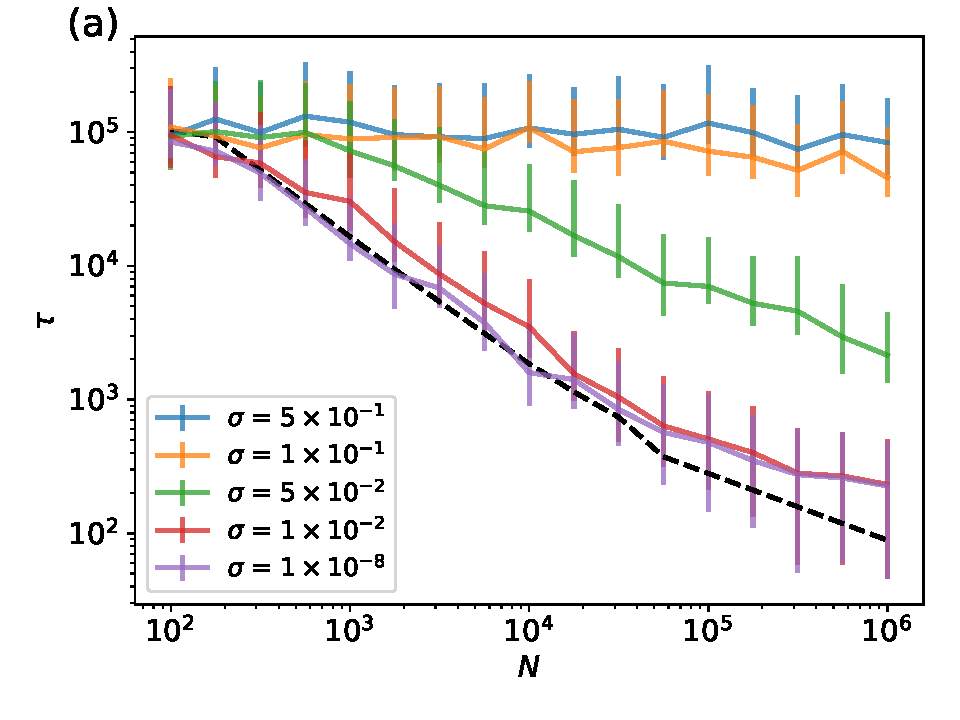
\includegraphics[width=0.48\textwidth]{Figures/julia_weissman_5a.pdf} &
%\label{fig:weissmana}
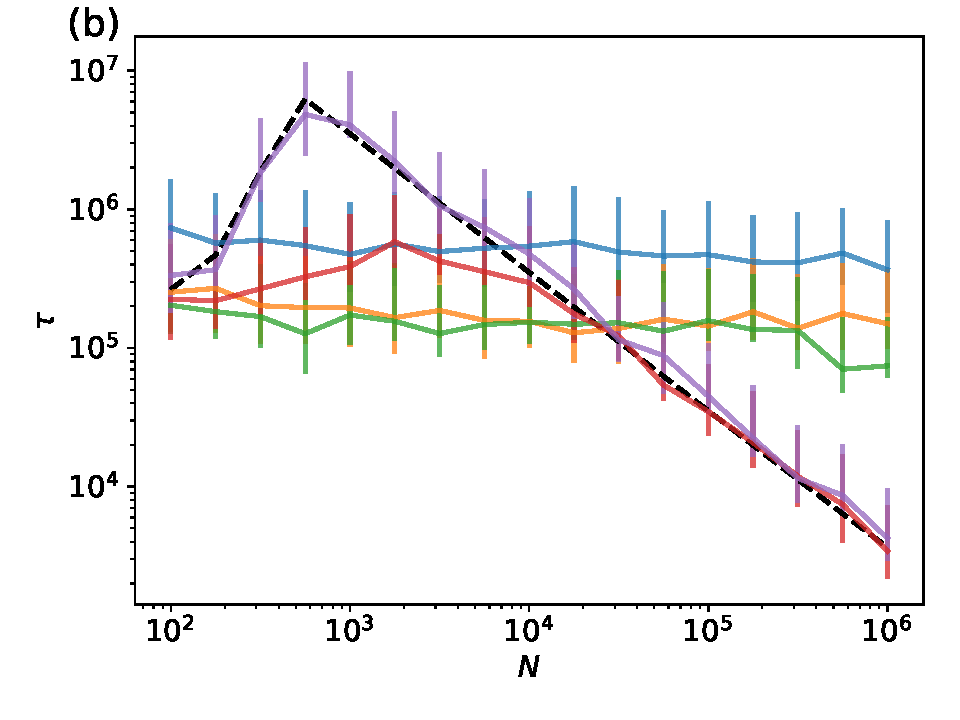
\includegraphics[width=0.48\textwidth]{Figures/julia_weissman_5b.pdf}\\[-3ex]
%\label{fig:weissmanb}
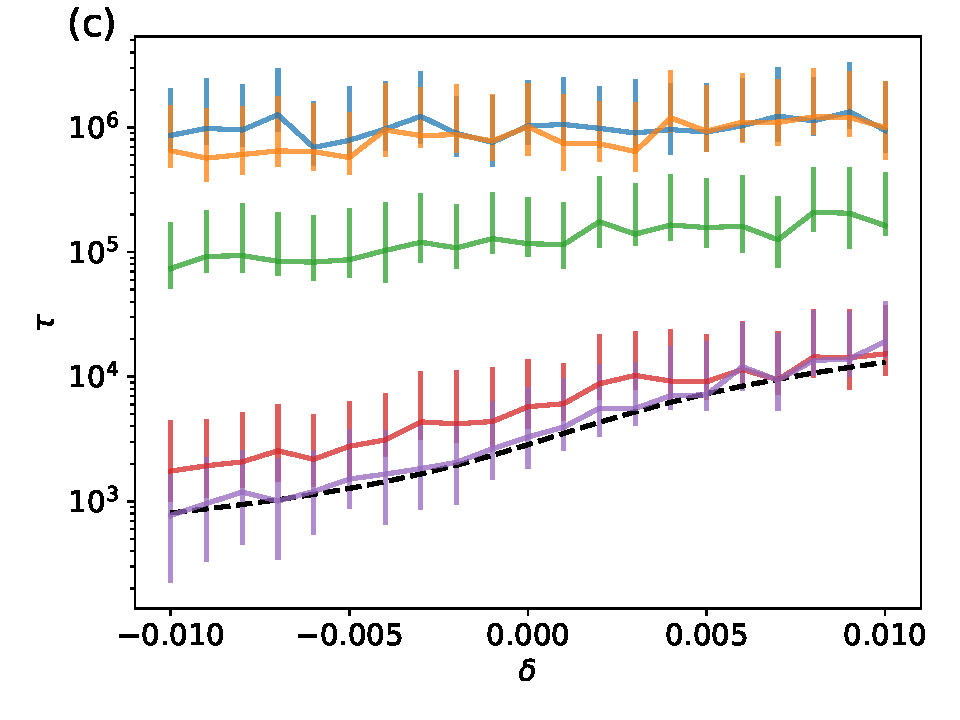
\includegraphics[width=0.48\textwidth]{Figures/julia_weissman_5c.pdf} &
%\label{fig:weissmanc}
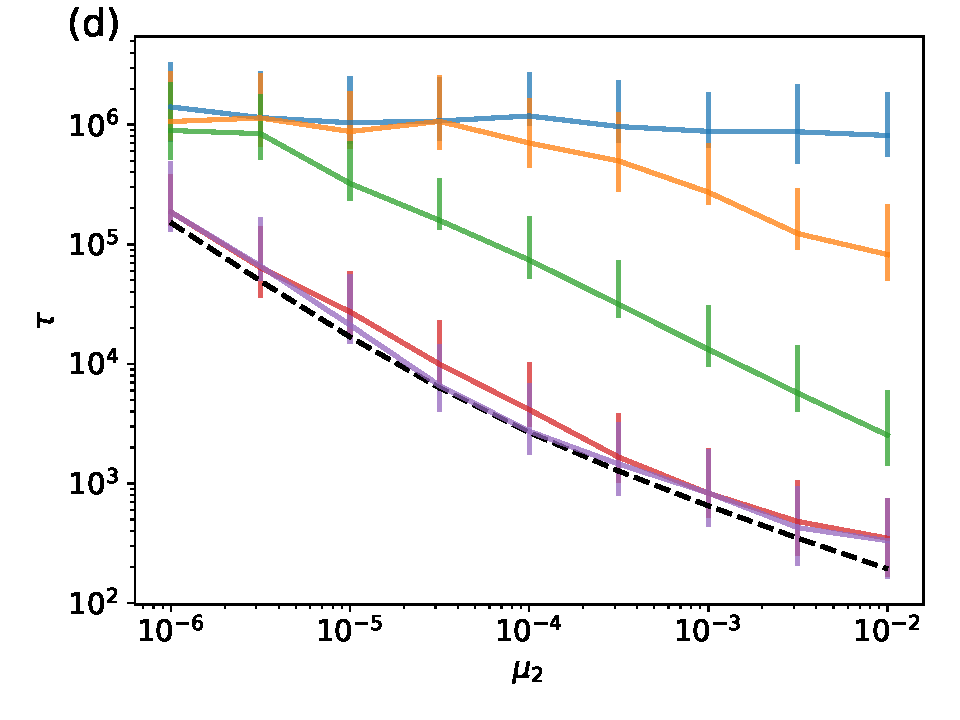
\includegraphics[width=0.48\textwidth]{Figures/julia_weissman_5d.pdf}
% \label{fig:weissmand}
  \end{tabular}
  \caption{Valley crossing times across a range of parameter values mirroring those of \citet{weissman_2009}. In each case, we set $s = 0.1$. In figures (a) and (b), the population size is varied: increasing the size causes valley crossing to transition from tunneling to semi-deterministic fixation. In (a), $\mu_1 = 10^{-5}$, $\mu_2 = 10^{-4}$, and $\delta = 2 \times 10^{-4}$, so that the valley depth is effectively neutral; in (b), $\mu_1 = 10^{-5}$, $\mu_2 = 10^{-6}$, and $\delta = 7 \times 10^{-3}$. In figure (c), we set $N = 10^5$, $\mu_1 = 10^{-6}$, and $\mu_2 = 4 \times 10^{-5}$. The valley depth $\delta$ is varied: at negative $\delta$, our simulations closely match the expectation for beneficial mutations. In figure (d), the intermediate mutation rate $\mu_2$ is varied, with $N = 10^{5}$, $\mu_1 = 10^{-6}$, and $\delta = 3 \times 10^{-3}$. Dotted lines represent the theoretical predictions from \citet{weissman_2009}.}
\label{fig:weissman}
\end{figure*}

Here we present the key results of our simulation analysis.
Figure \ref{fig:weissman} summarizes the major differences between the drift (low $\sigma$) and draft (high $\sigma$) regimes in valley crossing.
Note that the theoretical predictions differ slightly from those of \citet{weissman_2009} due to their use of a Moran model, compared to our modified Wright-Fisher model: this is comparable to an order of 2 difference in the population size.
The general trend is that draft causes valley crossing to take more time but be less sensitive to the underlying parameter values.
In figure \ref{fig:weissman}a, tunneling at low $\sigma$ occurs via neutral sequential fixation at low $N$ before transitioning into neutral tunneling and semi-deterministic tunneling at higher $N$; these are visible as minor kinks in the theoretical predictions (dotted line).
At low $\sigma$, our results agree with those predictions, but as $\sigma$ increases, the dependence on $N$ is lessened: at higher $\sigma$, the population effectively behaves as though there is a very small $N_e$, resulting in no dependence on $N$.
These trends are also visible in figure \ref{fig:weissman}c where, in the drift case, the population transitions from neutral to deleterious tunneling, and figure \ref{fig:weissman}d, in which deleterious tunneling gives way to neutral tunneling as the mutation rate $\mu_2$ increases.

One remarkable difference between drift and draft can be seen in figure \ref{fig:weissman}b.
At $\sigma = 10^{-8}$, crossing proceeds via deleterious sequential fixation at low $N$, then transitions into deleterious tunneling around $N = 10^3$ and semi-deterministic tunneling at higher $N$.
The increase in crossing time with $N$ is a hallmark of deleterious sequential fixation: higher $N$ means the deleterious intermediate is more ``visible" to selection, slowing its overall growth.
Once the population becomes large enough that fixation of the intermediate is unlikely, raising $N$ increases the number of single mutant ``bubbles" that are generated, resulting in the $\tau \sim N^{-1}$ crossing time dependence.
As $\sigma$ approaches even the moderate value $10^{-2}$, the crossing time curve flattens significantly; it still positively depends on $N$ but never approaches the peak crossing time $\approx 10^7$ generations in the $\sigma = 10^{-8}$ case.
The behavior in these two cases is qualitatively different: the intermediate $\sigma$ curve's dependence on $N$ cannot be reduced to the drift case simply by defining a reduced $N_e$.
In effect, from the point of view of the focal mutations, draft flattens the fitness landscape somewhat but not completely.
At higher values of $\sigma$, $\tau$ is again mostly independent of $N$, an indicator that sequential fixation is the dominant mode of crossing.

\begin{figure}[t]
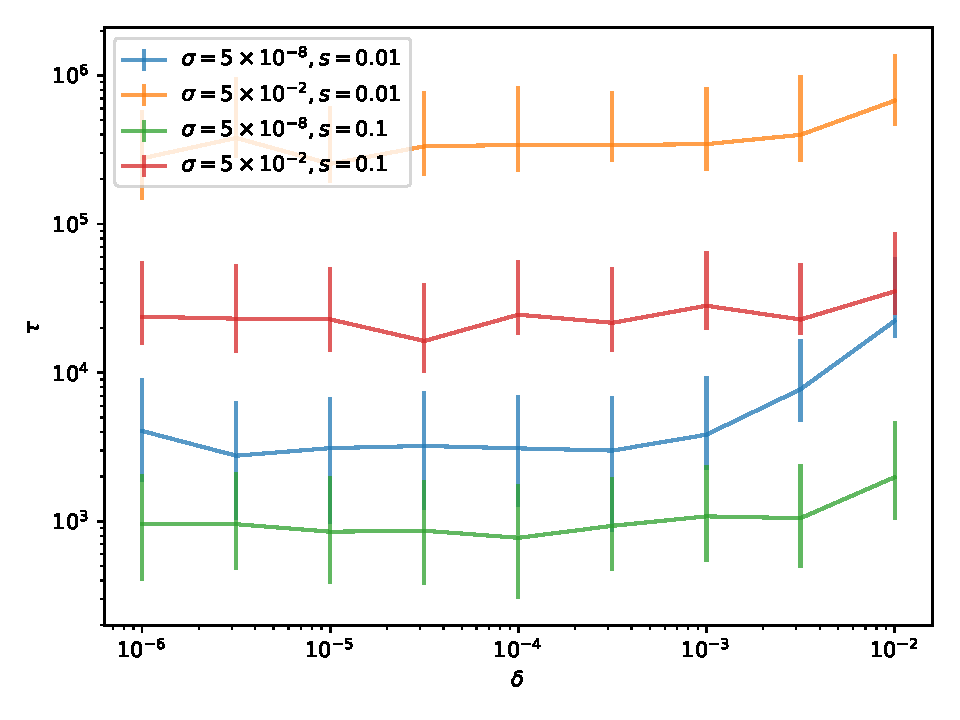
\includegraphics[width=0.5\textwidth]{Figures/julia_sigma_delta.pdf}
\caption{Valley crossing times for varied $\sigma$ and $\delta$. In these simulations, $N = 10^5$, $\mu_1 = 3 \times 10^{-6}$, and $\mu_2 = 10^{-4}$. Note the near lack of dependence on $\delta$ at high $\sigma$.}
\label{fig:sigma_delta}
\end{figure}

Overall, we find that $\tau$ is mostly elevated at high $\sigma$, as genetic draft dooms new lineages to extinction quickly and slows the growth of the complex adaptation.
On the other hand, the reduced effectiveness of selection should generally be helpful in crossing deeper valleys by mitigating the deleterious effect of single mutants.
This can be seen at intermediate values of $N$ in Figure \ref{fig:weissman}b and in figure \ref{fig:sigma_delta}.
At high values of $\sigma$, the fitness effect of the deleterious intermediate mutation has very little effect on the valley crossing time, which means that deep valleys can be crossed.
This suggests that traversing rugged fitness landscapes by valley crossing may be enhanced in rapidly adapting populations as landscapes under genetic draft appear to be ``flattened".

\begin{figure*}[t]
  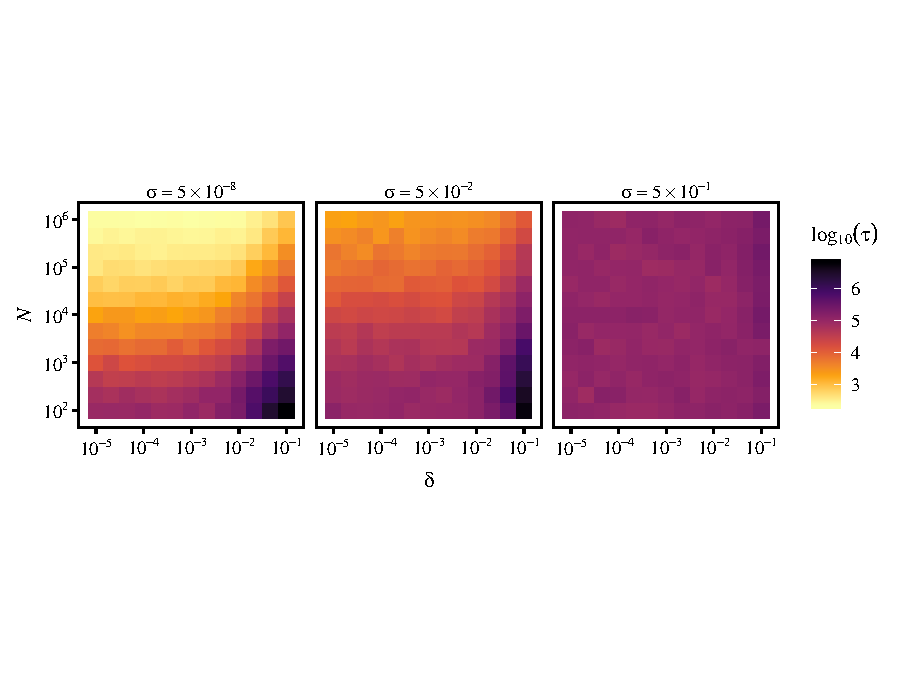
\includegraphics[width=\textwidth]{Figures/log_tau_s0-1.pdf}
  \caption{Valley crossing times on a $\log_{10}$ scale as a function of $\sigma$, $N$, and $\delta$. In all three plots, $s = 0.1$, $\mu_1 = 10^{-5}$, and $\mu_2 = 10^{-4}$.}
\label{fig:tau}
\end{figure*}
\begin{figure*}[t]
  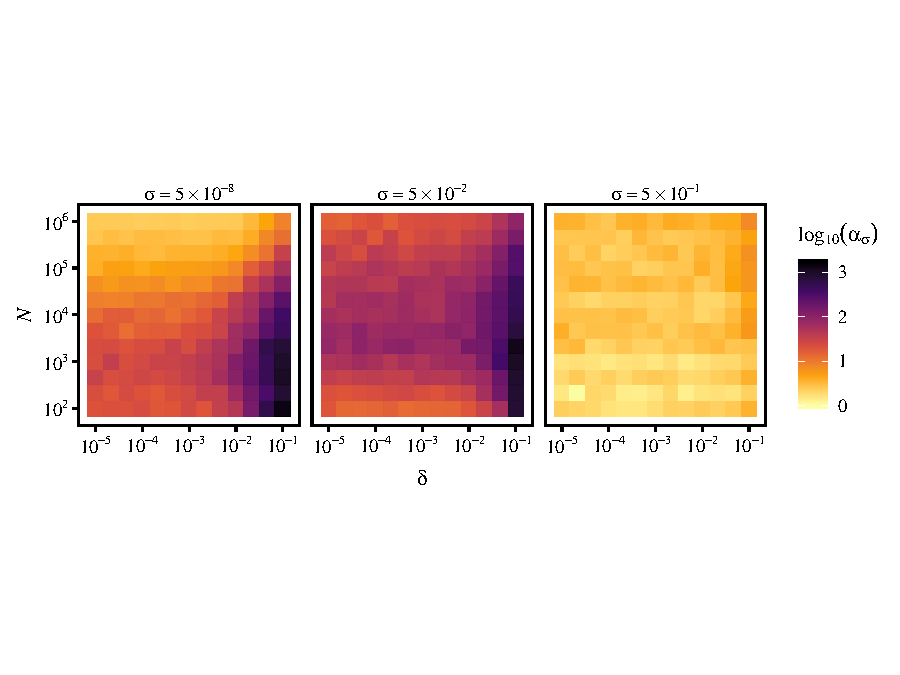
\includegraphics[width=\textwidth]{Figures/log_alpha_s0-1.pdf}
\caption{The ratio $\alpha = \tau_{\mathrm{valley}}/\tau_{\mathrm{sweep}}$ as a function of $\sigma$, $N$, and $\delta$. In all cases, $s_{\mathrm{sweep}} = 0.01$, $s_{\mathrm{valley}} = 0.1$, $\mu_1 = 10^{-5}$, and $\mu_2 = 10^{-4}$.}
\label{fig:tau-ratios}
\end{figure*}

So far, we can see that valley crossing is slower in rapidly adapting populations but the crossing time is less sensitive to the depth of the valley.
How do these two effects combine to shape the likelihood of valley crossing in rapidly adapting populations experiencing genetic draft compared to populations only experiencing drift?
To explore this, we first introduce the ratio $\alpha = \tau_{\mathrm{valley}}/\tau_{\mathrm{sweep}}$, where $\tau_{\mathrm{sweep}}$ is the time required for a single beneficial mutation to sweep to fixation and $\tau_{\mathrm{valley}}$ is the time required for a valley crossing event to occur.
By comparing how $\alpha$ changes as a function of the strength of selection on linked variation, $\sigma$, we can determine how $\sigma$ affects the speed of valley crossing relative to simple (``hard") selective sweeps. Higher (or lower) values of $\alpha$ mean that valley crossing times increase (or decrease) relative to the time required for a simple sweep.
Though the precise value of this ratio depends on $\delta$ and on the selection coefficients $s_{\mathrm{valley}}$ and $s_{\mathrm{sweep}}$ of the complex adaptation and the single beneficial mutation, respectively, a general trend nonetheless emerges.
In Figure \ref{fig:tau-ratios}, we set $s_{\mathrm{sweep}} = 0.01$, $s_{\mathrm{valley}} = 0.1$, $\mu_1 = 10^{-5}$, and $\mu_2 = 10^{-4}$.
Figure \ref{fig:tau-ratios} shows the expected pattern that deeper valleys in smaller populations take longer to cross.
At a higher value of $\sigma$, valley depth has a weaker effect on the valley crossing time in both an absolute sense (figure \ref{fig:tau}) and relative to the time for a single beneficial sweep (figure \ref{fig:ratios}).
Moreover, values of $\alpha$ are generally lower for the population with higher $\sigma$ experiencing genetic draft than for the population with lower $\sigma$ experiencing only drift.
This implies that draft tends reduce the valley crossing time relative to the time for a single beneficial mutation to sweep.

\begin{figure*}[t]
  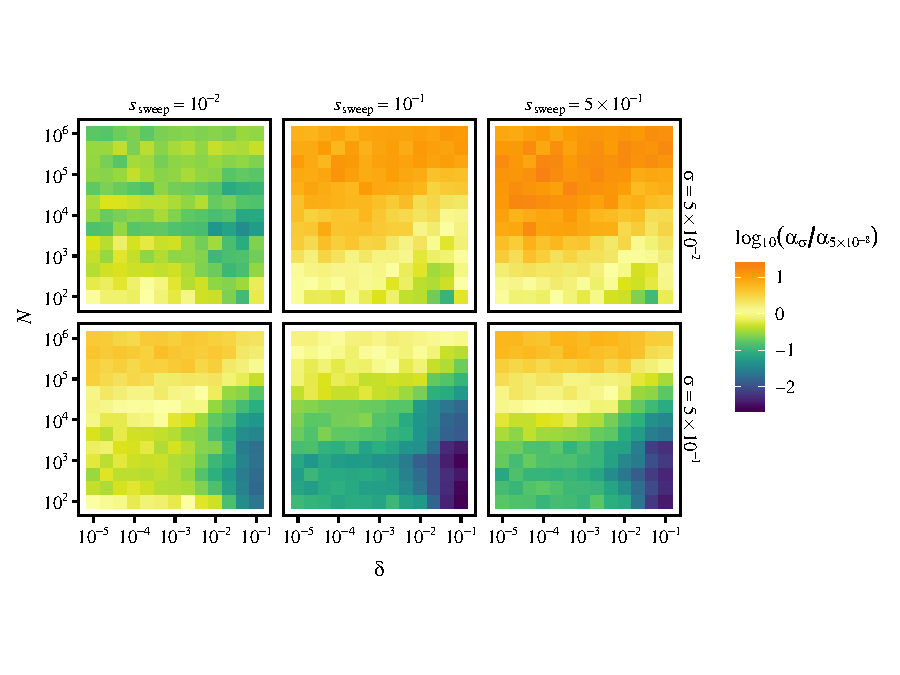
\includegraphics[width=\textwidth]{Figures/log_ratio_s0-1.pdf}
\caption{Ratio of $\alpha$ values at high and low $\sigma$ ($\log \left( \alpha_{\sigma_2} / \alpha_{\sigma_1} \right)$), where $\sigma_1=5 \times 10^{-8}$ and $\sigma_2$ values are on the right of the plot. $s_{\mathrm{sweep}}$ varies: other parameter values are as in figures \ref{fig:tau} and \ref{fig:tau-ratios}. A value lower than $0$ indicates that draft favors valley crossing. Genetic draft is helpful for crossing deep valleys, especially at low or intermediate sizes.}
\label{fig:alpha-ratios}
\end{figure*}


\begin{figure*}[t]
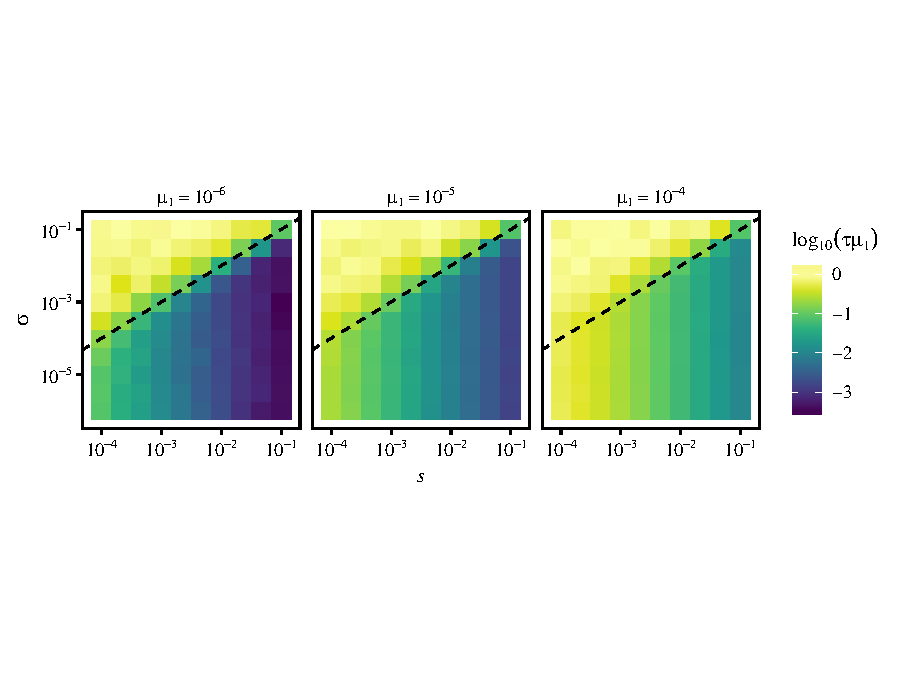
\includegraphics[width=\textwidth]{Figures/log_taumu.pdf}
\caption{The product of the crossing time $\tau$ and mutation rate $\mu_1$ at the first locus, as a function of $s$ and $\sigma$. The dotted line is $s = \sigma$. When $\sigma \gg s$, the genetic background dwarfs the fitness effect of the complex adaptation, and fixation is essentially neutral; when $\sigma \ll s$, the fixation time decreases with $s$. Note that, in the middle column, $s_{\mathrm{valley}} = s_{\mathrm{sweep}}$.}
\label{fig:tau-mu}
\end{figure*}

We can get a clearer picture of how draft affects valley crossing times relative to single beneficial sweeps by considering the ratio $\alpha_{\sigma_2} / \alpha_{\sigma_1}$ where $\sigma_1=5 \times 10^{-8}$ and $\sigma_2$ is allowed to vary.
This is a measure of the extent to which rapid adaptation speeds up valley crossing relative to sweeping (lower values indicate that rapid adaptation favors valley crossing).
The ratio can be seen in Figure \ref{fig:alpha-ratios}.
Overall, we find that raising $\sigma$ increases the extent to which valley crossing is favored, especially for lower population sizes.
In this regime, raising $\delta$ also increases the degree to which valley crossing is favored under draft, which means that the deeper the valley, the more that draft increases the likelihood of valley crossing relative to a single beneficial mutation.
The effect being exacerbated at low $N$ suggests that deleterious intermediates are surfing to very high frequency as the fitness wave advances.
The middle column is of special interest, as $s_{\mathrm{valley}} = s_{\mathrm{sweep}}$.

We further probe the effects of increasing $\sigma$ in Figure \ref{fig:tau-mu}.
At low values of $\sigma$, a strongly selected complex adaptation (high $s$) is essentially far ahead of the fitness wave and behaves as though governed by genetic drift, not draft.
This is consistent with the treatment of \citet{good_2012}, who found that, for beneficial lineages whose fitness $x + s$ is very far ahead of a critical fitness $x_c$, the fixation probability effectively scales with $x+s$.
Raising $\sigma$ far above $s$ (i.e., above the dotted line) causes the effect of $s$ to be overwhelmed by the advancing mean fitness, and fixation appears to be effectively neutral.

\section{Discussion}

We have used simulation methods to examine the rate of crossing fitness valleys in rapidly adapting populations that experience genetic draft.
We find that although the overall valley crossing time is longer in rapidly adapting than in slowly adapting (drifting) populations, a higher fraction of adaptive events in rapidly adapting populations may occur through valley crossing than in slowly adapting populations.
This mean that the genetic draft that results from rapid adaptation accelerates the rate at which populations escape from local peaks in a fitness landscape and move towards global peaks.
Thus, adaptation at loci unhindered by genetic draft occurs faster, but the population is more likely to get stuck on a local peak in a rugged fitness landscape.

The source of this difference in behavior between populations experiencing genetic draft and those experiencing drift comes from two effects.
First, the effect of the deleterious intermediate in the rapidly adapting population is much smaller: for $\delta \ll \sigma$, the precise value of $\delta$ does not affect the crossing rate.
Second, the time to the evolution of even \emph{simple} adaptations (i.e., ones requring substitution only at a single locus) is much longer in rapidly adapting populations.
This means that the presence of a fitness valley is not as steep of an impediment to the evolution of a complex adaptation for a drafting population as it is for a drifting one.

Our results complement and build on those of \citet{ochs_2015}, who compared valley crossing and a sweeping beneficial mutation in a slowly evolving population.
They considered the scenario where the sweeping beneficial mutation \emph{competes} with a particular complex adaptation, whereas we treat these two scenarios separately.
They find that large populations are more likely to cross valleys than fix a simple beneficial mutation than small populations (for comparison, see the $\sigma=5 \times 10^{-8}$ panel in our Figure \ref{fig:tau-ratios}).
However, they also find that intermediate-sized populations in which stochastic tunneling occurs are the least likely to cross a fitness valley instead of fixing a beneficial mutation.
In contrast, our results suggest that the stochastic tunneling regime is fairly narrow in rapidly adapting populations, and draft can aid the crossing of fitness valleys via sequential fixation of mutations.
Thus, it is possible that genetic draft improves the likelihood of valley crossing precisely where it is least likely under genetic drift. 

We have focused exclusively on asexual populations, but extensions to sexual populations are possible.
The relevant parameter is likely to be the product of $N$ and the proportion of the fitness standard deviation segregating in a small, effectively asexual block, $\sigma_b$ \citep{neher_kessinger_2013}.
If both $N\sigma$ and $N\sigma_b$ are large, and the focal loci segregate in the same block, then the analysis presented here should determine the crossing time.
If, on the other hand, $N\sigma$ is large but $N\sigma_b$ is small, or the map distance between the focal loci is much larger than the block length, then recombination between the focal loci can be modeled as ``free", with individuals effectively shuffling their entire genomes every generation.
In that case, the communal recombination analysis of \citet{neher_shraiman_2011} and \citet{neher_shraiman_2010} is likely to be important: the relationship between $\sigma$ and the recombination rate $\rho$ determines the crossing rate.
If $\sigma$ is large, then draft dominates the crossing rate: if $\rho$ is large, then drift dominates it.

One common feature of the effect of genetic draft and population subdivision on valley crossing is that they both increase the appearance of complex adaptations by reducing selection against deleterious intermediates (i.e., the valley genotypes).
In contrast, high migration rates and high recombination rates \citep{neher_shraiman_2009} allow selection to more easily remove deleterious intermediates.
This commonality has implications for Wright's ``shifting balance theory" \citep{Wright:1932}, which posits that population subdivision can enhance evolution on rugged fitness landscapes: deleterious intermediates accumulate due to genetic drift induced by subdivision, and subsequent beneficial mutations fix locally and are spread globally due to migration.
However, it has long been known that the shifting balance theory has important limitations due to the fact that too much migration prevents the accumulation of deleterious intermediates and too little reduces the success of genotypes from the fitter peaks and prevents them from spreading throughout the metapopulation \citep{coyne_barton_turelli_2000,Van-Cleve:Weissman:2015}.
Recent work by \citet{Bitbol:Schwab:2014} confirms the fact that intermediate migration rates yield the fastest valley crossing times; however, it also finds that valley crossing is faster in subdivided populations with these intermediate migration rates than in panmictic populations.

In light of our results that show that genetic draft can improve the likelihood of valley crossing, populations which experience both subdivision \emph{and} rapid adaptation are ideal candidates in which the shifting balance theory may apply.
Such populations include HIV, in which host-specific adaptations evolve quickly \citep{zhang_1997, wain_2007, dapp_2017, theys_2018} and in which deleterious mutations are known to hitchhike to high frequency \citep{zanini_2013, zanini_2015}.
Our work also shines light on the likely pathway through which multi-drug resistance evolves in HIV.
In recent years of the HIV pandemic, resistance has generally been slower to evolve \citep{feder_2015} because more and stronger drugs are used.
There are several possible explanations for this.
One is that the use of anti-HIV drugs decreases the number of virions segregating within an individual, thus lowering the number of possible chances for a resistant phenotype to appear.
Another is that such drugs, especially when used in concert, contort the fitness landscape so that evolution of a phenotype that is resistant to a drug cocktail is more difficult.
Both factors are likely to play a role.
However, since HIV is a population in which draft, not drift, is the dominant stochastic force and hence population size is less important in determining the evolutionary dynamics, our work suggests that the second factor is likely to be more significant in HIV compared to organisms in which draft is less important; indeed, the population size turns out to be less and less important as the effect of draft is ramped up.

Our results for the dynamics of valley crossing under genetic draft are likely to be important for other evolutionary problems in which stochastic forces are known to be important.
For example, there is a sort of duality between the evolution of complex adaptations and the evolution of cooperation, which can be seen as a complex behavioral adaptation where the highest per capita fitness at equilibrium requires the combination of multiple cooperative individuals (i.e., the combination of genes among different individuals instead among different loci).
In social evolution theory, high migration rates between demes, which cause organisms to be less likely to interact with close kin, disfavor the evolution of cooperation: likewise, when migration rates are low, cooperation can be favored \citep{Hamilton:1970,Rousset:2004,van_cleve_2015}.
Evolutionary forces which strengthen existing associations between loci are more likely to lead to such complex phenotypes: evolutionary forces which weaken these associations hinder their evolution.
This reasoning applies whether the loci in question appear in the same individual (as in the case of sign epistasis) or in different individuals (as in the case of social evolution).
These effects can even interact: cooperation can function as an additional evolutionary force that favors valley crossing \citep{Obolski:Lewin-Epstein:2017} and can in some cases be a valley crossing adaptation in itself \citep{van_cleve_2013}.
The interplay between cooperation and valley crossing is an area that needs further study, as it may shed light on the evolution of cooperation within large microbial populations such as yeast \citep{gore_2009, gore_2013} and bacterial biofilms \citep{rainey_2003, van_gestel_2014}.


\section*{Acknowledgments}

This work is supported by the National Science Foundation under Cooperative Agreement No. 1355438.

\bibliography{bib}

\end{spacing}

\end{document}